\documentclass[conference]{IEEEtran}
\IEEEoverridecommandlockouts
% The preceding line is only needed to identify funding in the first footnote. If that is unneeded, please comment it out.
\usepackage{cite}
\usepackage{amsmath,amssymb,amsfonts}
\usepackage{algorithmic}
\usepackage{graphicx}
\usepackage{textcomp}
\usepackage{xcolor}
\usepackage{float}

% A todo macro for marking ToDos
\usepackage{color}
\newcommand{\todo}[1]{\textcolor{white}{\colorbox{blue}{ To do %
			:}}\textcolor{blue}{\ \ #1
	}\textcolor{blue}{\colorbox{blue}{III}}\ }
%\renewcommand{\todo}[1]{}

\def\BibTeX{{\rm B\kern-.05em{\sc i\kern-.025em b}\kern-.08em
    T\kern-.1667em\lower.7ex\hbox{E}\kern-.125emX}}
\begin{document}

\title{Projektdokumentation Smartstall\\
}

\author{\IEEEauthorblockN{1\textsuperscript{st} Hannes Bruhn}
\IEEEauthorblockA{\textit{Hochschule für angewandte Wissenschaften Coburg} \\
hannes\_bruhn@web.de}
\and
\IEEEauthorblockN{2\textsuperscript{nd} Florian Wermbter}
\IEEEauthorblockA{\textit{Hochschule für angewandte Wissenschaften Coburg} \\
florianwermbter@gmail.com}
}

\maketitle

\begin{abstract}
Hier steht das Abstract.
\end{abstract}

\begin{IEEEkeywords}
component, formatting, style, styling, insert
\end{IEEEkeywords}

\section{Hintergrund und Ziel des Projekts}
Das Projekt Smartstall ist im Rahmen des Moduls "Hardware cypher-physischer Systeme" des Master-Studiengangs Informatik entstanden, bei dem es um Schnittstellen und Datenübertragung von Endgeräten, sowie die Anbindung dieser an die Cloud nach dem Internet of Things (IoT) Konzept geht. \\
Ziel dieses Projekts ist die Erfassung unterschiedlicher Sensordaten zur Überwachung der Luftqualität in einem Stall. Die erfassten Daten sollen über einen Raspberry Pi an eine, für dieses Projekt entwickelte Webanwendung gesendet werden. Dadurch soll der Anwender die Möglichkeit erhalten, die Daten über eine benutzerfreundliche Oberfläche anzuzeigen und zu analysieren. Bei der Überschreitung von festlegbaren Schwellwerten bestimmter Attribute wie Temperatur, Luftfeuchtigkeit oder Ammoniakgehalt, soll der Anwender außerdem per Push-Up Benachrichtigung auf seinem Smartphone informiert werden können. \\
Des Weiteren soll die Belüftung von der Webanwendung bei Bedarf ein- und ausgeschaltet werden können, um die Schwellwerte auch ohne aktives Eingreifen des Anwenders wieder unterschreiten zu können. Dies soll durch die Ansteuerung einer WLAN-Steckdose umgesetzt werden. Durch regelmäßige und kontinuierliche Datenerfassung wird dafür gesorgt, dass die Belüftung nur so lange wie nötig aktiviert ist, womit die Aspekte Effizienz und Nachhaltigkeit berücksichtigt und in das Projekt integriert werden. 

\section{Überblick}
%sowas wie aufbau der doku

\section{Anforderungserhebung}
\subsection{Ursprüngliche Überlegungen}
Das Ziel von SmartStall ist die Kontrolle der Luftqualität in einem Stall. Durch den Einsatz von Sensoren sollen Ammoniak, Temperatur und Luftfeuchtigkeit überwacht werden, um sicherzustellen, dass diese Werte nicht in schädliche Bereiche gelangen. Da die Umrüstung auf eine neue smarte Belüftung sehr kostspielig sein kann, soll SmartStall eine kostengünstige Alternative bieten.
Die erfassten Luftqualitätsdaten sollen in Diagrammen für einen Tag und eine Woche in einer Webanwendung visualisiert werden. Diese Webanwendung soll mit einem Login, bei dem Benutzername und Passwort eingegeben werden muss, geschützt werden. In den Diagrammen soll die Grenzen, ab denen die einzelnen Luftdaten schädlich werden, rot markiert sein. Neben den aktuellen Daten sollen auch die durchschnittlichen Werte für eine Woche und einen Tag angezeigt werden. Es gibt insgesamt drei Diagramme: eines für Ammoniak, eines für Temperatur und eines für Luftfeuchtigkeit
Der Landwirt soll eine Push-Benachrichtigung erhalten, wenn ein Schwellwert überschritten wird, und die Belüftung soll automatisch eingeschaltet werden. Sobald alle Werte unter den Schwellwerten liegen, soll die Belüftung wieder ausgeschaltet werden.
Es ist von großer Bedeutung, dass die Werte für Ammoniak, Luftfeuchtigkeit und Temperatur in einem Stall nicht zu hoch sind. Hohe Ammoniakkonzentrationen können die Atemwege der Tiere und Menschen reizen und zu ernsthaften gesundheitlichen Problemen führen. Eine zu hohe Luftfeuchtigkeit kann das Wachstum von Schimmel und anderen schädlichen Mikroorganismen fördern, was wiederum die Gesundheit der Tiere beeinträchtigt. Extreme Temperaturen, ob zu hoch oder zu niedrig, können den Komfort und das Wohlbefinden der Tiere negativ beeinflussen, was zu Stress und einer verminderten Produktivität führen kann. Daher soll die Überwachung und Regelung dieser Parameter essenziell für die Gesundheit und das Wohlbefinden der Tiere sowie für eine effiziente landwirtschaftliche Produktion sein. 
Nach den ersten Überlegungen zu dem Projekt SmartStall wurde folgende Skizze zu einem möglichen Userinterface entwickelt:
%Bild einfügen
\subsection{Gespräch mit Landwirten}
Da SmartStall ein IT-Produkt für Landwirte mit Stalltieren werden soll, wurde nach den ersten Überlegungen und der ersten Skizze ein Gespräch mit zwei verschiedenen Landwirten geführt. Der erste landwirtschaftliche Betrieb ist der Bauernhof Stenglein in Rothwind, der etwa 80 Kühe in einem Stall hält. Der zweite landwirtschaftliche Betrieb ist der Bauernhof der Familie Stark aus Eichberg, die in der Ferkelerzeugung tätig sind. Beide reagierten positiv auf die Idee von SmartStall und fanden die Grundidee gut, brachten jedoch einige Verbesserungsvorschläge und wichtige Anmerkungen ein:
Die Landwirte waren der Meinung, dass es wenig Sinn macht, die durchschnittlichen Werte der einzelnen Luftqualitätsdaten anzuzeigen, da diese wenig aussagekräftig sind. Als Beispiel nannten sie die Temperatur: Im Sommer ist diese sehr hoch, im Winter eher niedrig. Ein Mittelwert daraus liefert keine nützlichen Informationen im Vergleich zum aktuellen Wert. Der Mittelwert wäre nur dann sinnvoll, wenn der Stall das ganze Jahr über konstante Bedingungen hätte, wie gleiche Außentemperatur und gleiche Dauer von geöffneten bzw. geschlossenen Türen und Fenstern, was in der Praxis jedoch nicht vorkommt. Da die Stalltüren ab spätem Frühling meist bis Herbst fast durchgängig geöffnet sind, herrschen unterschiedliche Bedingungen im Stall. Aus diesem Grund kann der durchschnittliche Wert der einzelnen Daten aus den Diagrammen entfernt werden, was zusätzlich die Lesbarkeit der Diagramme verbessert.
Den Landwirten war es außerdem wichtig, dass sie die Steuerung der Belüftung und die Push-Benachrichtigungen kontrollieren können. Da es sich um ein erstmaliges Projekt handelt, das noch nicht im Einsatz war, möchten sie sich nicht vollständig auf das System verlassen und die Möglichkeit haben, wie gewohnt vorzugehen.
Ein weiterer Verbesserungsvorschlag war das Hinzufügen des aktuellen Werts zu jedem Diagramm, damit man auf einen Blick den aktuellen Zustand im Stall erkennen kann.
Da der Bauernhof der Familie Stenglein recht groß ist und auch Angestellte im Stall arbeiten, die nicht viel mit Technik zu tun haben, wenig davon verstehen und nicht gut Deutsch sprechen, war es ihnen wichtig, dass die Anwendung simpel gehalten wird, damit sie theoretisch jeder bedienen und verstehen kann.
\subsection{Resultat
}Das Resultat des Projekts SmartStall ist wie folgt:
Die Luftqualitätsdaten des Stalls werden über einen Raspberry Pi in eine Datenbank geschrieben. Diese Daten werden in einer passwortgeschützten Webanwendung visualisiert, die drei verschiedene Diagramme enthält: eines für Ammoniak, eines für Luftfeuchtigkeit und eines für Temperatur. Die Diagramme zeigen die aktuellen Werte des Tages bzw. der letzten sieben Tage an. Die durchschnittlichen Werte für Tag und Woche wurden entfernt, um die Lesbarkeit zu verbessern.
Neben den Diagrammen wird der aktuelle Wert angezeigt, der in roter Schrift dargestellt ist, wenn der Wert die schädliche Grenze überschreitet, und in grüner Schrift, wenn er im unkritischen Bereich liegt. Es gibt außerdem zwei Schalter, mit denen die Automatisierung der Belüftung und das Benachrichtigen per Push-Nachricht bei Überschreitung des Grenzwerts aktiviert werden können.
Die Push-Benachrichtigungen werden an eine Telegram-Gruppe gesendet, in die alle Mitarbeiter eines Bauernhofs aufgenommen werden können, sodass jeder informiert ist. Eine Benachrichtigung wird auch gesendet, wenn die Steuerung der Belüftung deaktiviert wird, woraufhin das System die Belüftung abschaltet. Dies verhindert, dass die Belüftung unnötig lange läuft, falls sie zum Zeitpunkt der Deaktivierung noch aktiv ist, und trägt dazu bei, den Energieverbrauch des Stalls zu reduzieren. In Kapitel xy wird genauer auf das finale Userinterface eingeangen.



\section{Hardware Komponenten}
\subsection{Raspberry Pi 3B}
Der Raspberry Pi (Modell 3B) ist ein beliebter Einplatinencomputer, der von der Raspberry Pi Foundation entwickelt wurde. Er bietet ausreichend Rechenleistung, Speicher und Konnektivität, um komplexe Aufgaben auszuführen und eine Vielzahl von Erweiterungen und Anwendungen zu unterstützen und ist somit ein kostengünstige und vielseitige Plattform für Projekte im Bereich der Einbettung von Computern und des IoT. Die umfangreiche Community und Dokumentation rund um den Raspberry Pi machen es einfach, Projekte zu starten und Unterstützung zu erhalten. Es gibt eine Vielzahl von Erweiterungsmodulen und Zubehörteilen, die den Raspberry Pi erweitern und an individuelle Anforderungen anpassen können. Um den Raspberry Pi 3B zu nutzen, ist eine grundlegende Einrichtung erforderlich, auf welche in Kapitel \ref{pi} genauer eingegangen wird. \cite{raspy} 

\subsection{Bosch Sensortec BME680 Sensor}
Der Bosch Sensortec BME680 ist ein fortschrittlicher Umweltsensor, der verschiedene Messungen in einer kompakten Einheit vereint. Der BME680 Sensor ermöglicht die Messung von vier Umweltparametern:
\begin{itemize}
	\item Temperatur: Der Sensor misst die Umgebungstemperatur mit hoher Präzision.
	\item Luftfeuchtigkeit: Er erfasst die relative Luftfeuchtigkeit und liefert genaue Feuchtigkeitswerte.
	\item Luftdruck: Der Sensor kann den atmosphärischen Druck messen und damit Wettervorhersagen ermöglichen.
	\item Luftqualität: Der BME680 Sensor ist in der Lage, flüchtige organische Verbindungen (VOCs) und verschiedene Gase wie Kohlenmonoxid (CO) und Stickstoffdioxid (NO2) zu erkennen.
\end{itemize}
Der BME680 Sensor findet Anwendung in einer Vielzahl von Bereichen, wie beispielsweise der Erfassung von Wetterdaten in Außenbereichen und der Überwachung von Luftqualität in Innenräumen. \cite{bme}
\subsection{MQ137 NH3-Gassensormodul}
Das MQ137 Gassensor-Modul ist ein Sensor, der speziell entwickelt wurde, um Ammoniakgas (NH3) in der Umgebungsluft zu messen. Er basiert auf der Metalloxid-Gassensortechnologie und erfasst die Konzentration von Ammoniak in Parts per Million (ppm). Der Sensor reagiert auf das Vorhandensein von Ammoniak, indem er Änderungen in der elektrischen Leitfähigkeit erkennt. Das MQ137 Gassensor-Modul ermöglicht eine präzise Erfassung von Ammoniakgas und findet Anwendung in verschiedenen Bereichen wie Industrie, Landwirtschaft und Umweltüberwachung.

\subsection{Verbinden der Komponenten}
Um die vorgestellten Sensoren nutzen zu können, müssen diese an die korrekten Pins des Raspberry Pis angeschlossen werden. Die zur Verfügung stehenden Pins des Raspberry Pis sind in Abbildung \ref{pi_pins} dargestellt.

\begin{figure}[H]
	\centering
	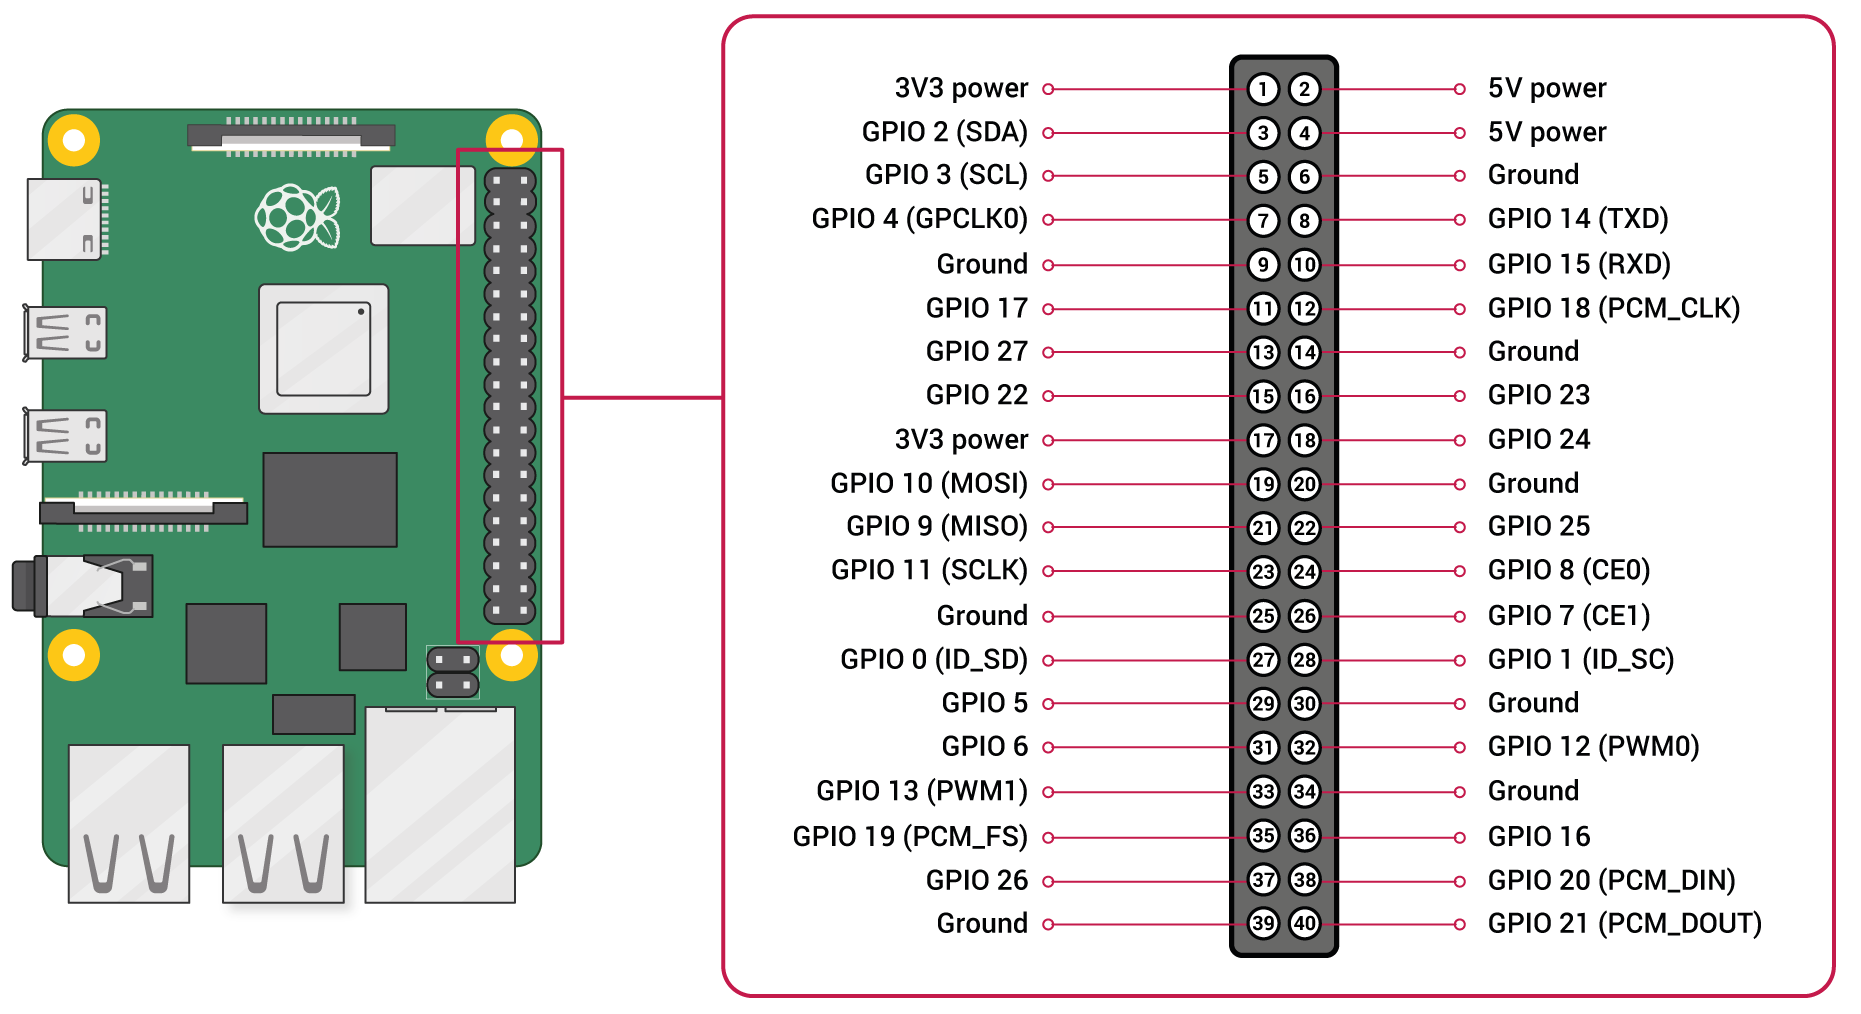
\includegraphics[width=90mm]{fig/pi_pins.png}
	\caption{Raspberry Pi 3B Pin Belegung}
	\label{pi_pins}
\end{figure}

\subsubsection{Anschließen des BME680 Sensors} 


Der BME680 besitzt sechs Pins, welche Abbildung \ref{bme_pins} zu entnehmen sind. Relevant sind hierbei die oberen 4 Pins, welche wie in Abbildung \ref{verkabelung_bme} aufgezeigt an den Raspberry Pi angeschlossen werden müssen. \cite{bme_anschluss}
\begin{figure}[H]
	\centering
	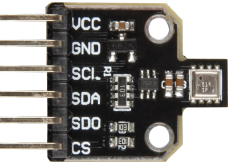
\includegraphics[width=50mm]{fig/bme_pins.png}
	\caption{BME680 Pins}
	\label{bme_pins}
\end{figure}
\begin{figure}[H]
	\centerline{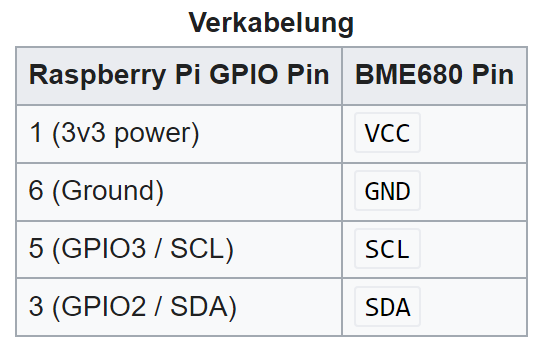
\includegraphics[width=50mm]{fig/verkabelung_bme.png}}
	\caption{Pin Verbindungen von Raspberry Pi und BME680}
	\label{verkabelung_bme}
\end{figure}

\subsubsection{Anschließen des MQ137 Sensors} 

Der MQ137 Sensor besitzt, wie in Abbildung \ref{mq137_pins} zu sehen 4 Pins, welche ebenfalls mit den jeweiligen Pins des Raspberry Pis verbunden werden müssen:
\begin{itemize}
	\item VCC: Stromversorgung (5V)
	\item GND: Ground
	\item DO: digitaler Signalausgang
	\item AO: analoger Signalausgang
\end{itemize}
\begin{figure}[H]
	\centerline{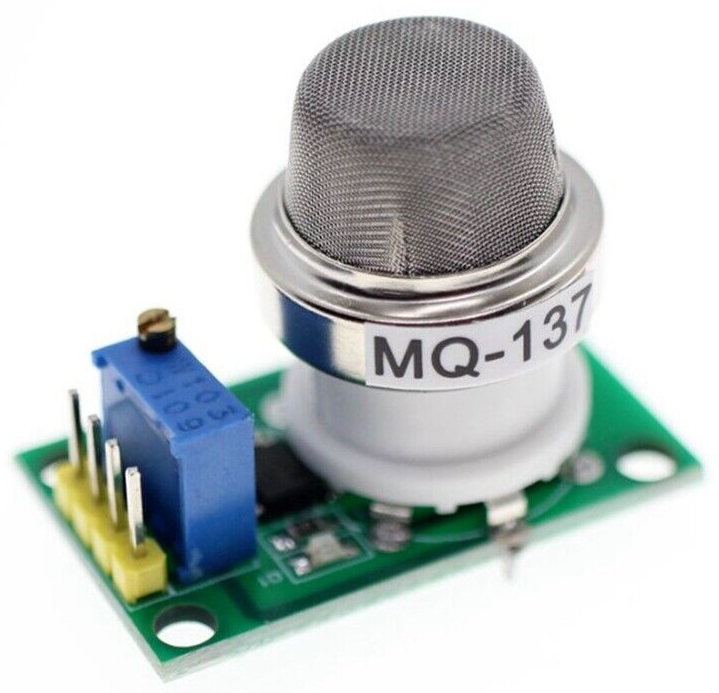
\includegraphics[height=40mm]{fig/mq137_pins.png}}
	\caption{MQ137 Gassensormodul}
	\label{mq137_pins}
\end{figure}

\subsubsection{Gesamtaufbau}
Die Sensoren wurden mittels Jumper-Kabeln und einem Breadboard mit dem Raspberry Pi verbunden. Der Aufbau und die beschriebene Verkabelung der Sensoren mit dem Raspberry Pi ist Abbildung \ref{aufbau} zu sehen.

\begin{figure}[htbp]
	\centerline{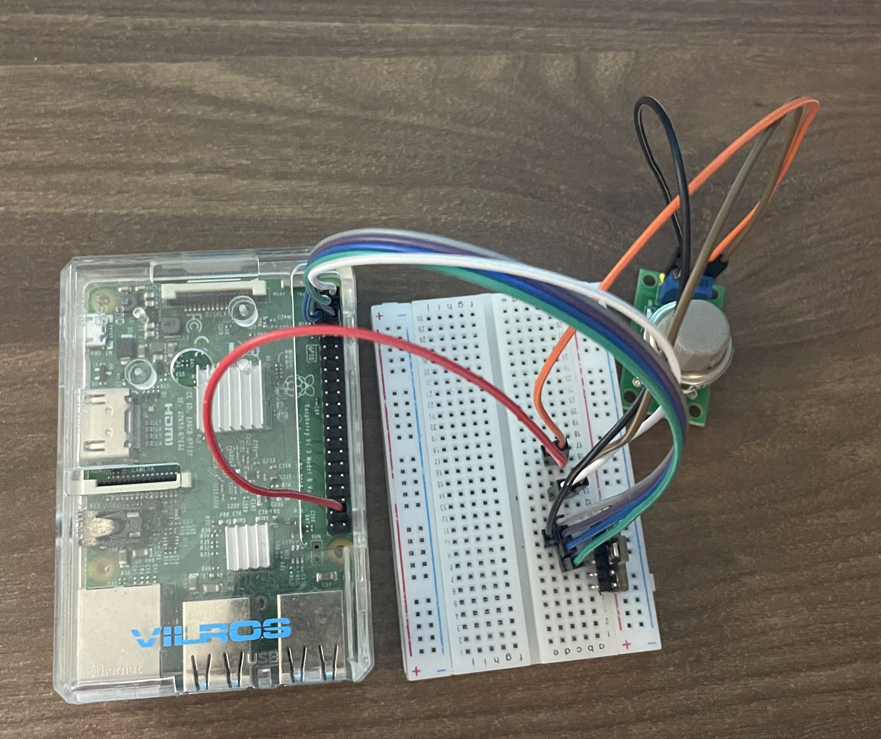
\includegraphics[width=80mm]{fig/aufbau.png}}
	\caption{Verkabelung der Sensoren mit dem Raspberry Pi}
	\label{aufbau}
\end{figure}

\section{Einrichtung Raspberry Pi}
\label{pi}
\subsection{Konfiguration}
Die erstmalige Einrichtung eines Raspberry Pi 3B umfasst mehrere Schritte, welche in diesem Kapitel aufgelistet werden. Zunächst eine Auflistung der benötigten und in diesem Projekt verwendeten Komponenten:
\begin{itemize}
	\item Raspberry Pi 3B
	\item MicroSD-Karte (mindestens 8 GB)
	\item Netzteil (5V)
	\item USB-Tastatur und -Maus
	\item HDMI-Kabel
	\item Bildschirm oder Fernseher mit HDMI-Eingang
\end{itemize}
Wenn das Anschließen von Ein- und Ausgabegeräten an den Raspberry Pi nicht gewünscht oder möglich ist, kann dieser nach der ersten Einrichtung alternativ auch über einen anderen Computer angesteuert werden, entweder per Remotedesktopverbindung oder per Kommandozeile mit Hilfe des Secure Shell (SSH) Netzwerkprotokolls. \cite{raspy} Zur erstmaligen Einrichtung muss zunächst das gewünschte Betriebssystem für den Raspberry Pi heruntergeladen werden, in diesem Fall Raspbian. Hierfür wurde das Program Raspberry Pi Imager von der offiziellen Raspberry Pi Website verwendet, welches die ausgewählte Version des Betriebssystems herunterlädt und diese direkt auf der MicroSD-Karte installiert. Anschließend kann die MicroSD-Karte in den Raspberry Pi eingesetzt und dieser gestartet werden. Für die Einrichtung muss nun lediglich den Anweisungen auf dem Bildschirm gefolgt werden, anschließend kann der Raspberry Pi über die grafische Benutzeroberfläche verwendet oder über Konsole angesteuert werden.  


\subsection{Software und Bibliotheken}
Nach der Einrichtung des Raspberry Pi musste zunächst das I2C (Inter-Integrated Circuit) Interface über die raspi-config aktiviert werden. I2C  ist ein serieller Kommunikationsbus zur Verbindung von elektronischen Bauteilen über nur zwei Datenleitungen: SDA (Serial Data Line) und SCL (Serial Clock Line). Es ermöglicht die einfache Kommunikation zwischen verschiedenen Geräten wie Mikrocontrollern, Sensoren und Aktoren. Dieser wird vom BME680 Sensor zur Übertragung der Messwerte genutzt. Da für das Abfragen der Sensordaten in diesem Projekt Python verwendet wird, welches bereits standardmäßig mit dem Raspian Betriebssystem mitinstalliert wird, müssen zusätzlich noch einige Bibliotheken installiert werden: 
\begin{itemize}
	\item python3-smbus: Ermöglicht die Kommunikation über in I2C-Bus in Python. Es werden Funktionen bereitgestellt I2C-Geräte anzusprechen und Daten zu senden und zu empfangen.
	\item i2c-tools: Wird für die Verwaltung und Diagnose des I2C-Busses verwendet. Dies bietet zusätzliche Funktionalitäten wie das Anzeigen angeschlossener Geräte.
	\item adafruit-circuitpython-bme680: 
\end{itemize}

\subsection{Datenübertragung}


\section{Webanwendung}
\subsection{Architektur und Design}
\subsection{Empfangen der Daten}
\subsection{Anbindung einer MYSQL Datenbank}
\subsection{Auslesen und Anzeigen der Sensordaten}
Für die Anzeige der Sensordaten in einer Webanwendung wurden bestimmte Anforderungen definiert. Zum einen sollten die Daten in einem Liniendiagramm dargestellt werden, und zum anderen sollte die Webanwendung sowohl auf PCs und Laptops als auch auf mobilen Geräten reibungslos funktionieren. Dies erforderte die Nutzung eines responsiven Frameworks wie Bootstrap.
Bootstrap wurde gewählt, da es eine breite Palette an vorgefertigten UI-Komponenten und ein responsives Grid-System bietet. Dies ermöglicht eine einfache Integration und schnelle Entwicklung von modernen und benutzerfreundlichen Webseiten, unabhängig vom verwendeten Gerät.
Um Bootstrap effektiv zu nutzen, wurden folgende JavaScript-Bibliotheken integriert:
jQuery: Diese leistungsstarke Bibliothek unterstützt die Manipulation des DOM und erleichtert AJAX-Interaktionen. In Verbindung mit Bootstrap ermöglicht sie die dynamische Aktualisierung von Inhalten und die Interaktion mit Benutzeroberflächenelementen wie Dropdown-Menüs oder Modalfenstern.
\begin{verbatim}
<script src="https://code.jquery.com/
jquery-3.6.0.min.js"></scrip
\end{verbatim}
Popper.js: Diese Bibliothek wird verwendet, um Popups, Tooltips und Dropdown-Menüs präzise innerhalb einer Bootstrap-Anwendung zu positionieren. Dies verbessert die Benutzerfreundlichkeit und sorgt für eine optimale Platzierung basierend auf dem verfügbaren Bildschirmraum
\begin{verbatim}
<script src="https://cdn.jsdelivr.net/
npm/popper.js@1.16.1/dist/umd/popper.min.
js"></script>
\end{verbatim}
Bootstrap: Das Bootstrap-Bundle enthält das Haupt-JavaScript von Bootstrap sowie die erforderlichen Abhängigkeiten wie jQuery und Popper.js. Diese Kombination bietet Funktionen wie responsives Design, Grid-Systeme und Modalkomponenten, die für die Implementierung des Liniendiagramms und anderer UI-Elemente essentiell sind.
\begin{verbatim}
<script src="https://cdn.jsdelivr.net/
npm/bootstrap@4.6.2/dist/js/bootstrap.
bundle.min.js"></script>
\end{verbatim}
Zusammen stellen diese Skript-Links sicher, dass Bootstrap nahtlos in die Webanwendung integriert wird und eine optimale Benutzerinteraktion sowie eine responsive Darstellung auf verschiedenen Geräten gewährleistet ist.
Für die Darstellung der Sensordaten in einem Liniendiagramm wurde Chart.js gewählt. Diese Bibliothek bietet eine einfache und flexible Möglichkeit, Daten visuell ansprechend darzustellen. Im Vergleich zu Grafana, das eher für umfangreichere und komplexe Datenvisualisierungen in großen Systemen verwendet wird, ist Chart.js leichter in kleinere Webanwendungen zu integrieren und bietet dennoch ausreichend Funktionalität für die Anforderungen der Sensordatenvisualisierung.
Die folgenden Links integrieren Chart.js und das zugehörige Datum-Adapter-Bundle in die Webseite:
\begin{verbatim}
<script src="https://cdn.jsdelivr.net/npm/
chart.js"></script>
<script src="https://cdn.jsdelivr.net/npm
/chartjs-adapter-date-fns/dist/chartjs-
adapter-date-fns.bundle.min.js"></script>
\end{verbatim}
Diese Entscheidungen zusammen ermöglichen eine effektive und effiziente Darstellung der Sensordaten in der Webanwendung, optimiert für verschiedene Geräte und Benutzerumgebungen.
Nachdem die benötigten Bibliotheken eingebunden wurden, kann das Diagramm für die Temperatur in der Webanwendung aufgebaut werden. Der  HTML-Code in Anhang xy definiert die Struktur des Diagramms.

Das eigentliche Diagramm wird durch das \texttt{<canvas>}-Element mit der ID \texttt{lineChartTemperatur} dargestellt.
Um die Sensordaten für die Temperatur abzurufen, wird AJAX verwendet. AJAX ermöglicht es, Daten asynchron im Hintergrund zu laden, ohne die gesamte Webseite neu zu laden. Der JavaScript-Code in Anhang xy zeigt einen Beispielaufruf.

Hierbei ist \texttt{GetTemperatur} die URL, unter der die Sensordaten abgerufen werden. Die empfangenen Daten werden in ein JavaScript-Dictionary umgewandelt (\texttt{temperaturWerteTagAktuellDictionary}), um sie später im Diagramm anzuzeigen.
Die Verwendung von AJAX ist besonders nützlich, da sie eine flüssige Benutzererfahrung ermöglicht, indem Daten im Hintergrund geladen werden, während die Benutzeroberfläche weiterhin interaktiv bleibt. Dies ist wichtig für die dynamische Aktualisierung und Visualisierung von Echtzeitdaten wie den Sensormessungen der Temperatur.
In der Funktion createTemperaturDiagramTag wird das Diagramm erstellt, wobei die Sensordaten entsprechend bearbeitet werden müssen. Die folgenden Codeabschnitte sind hierbei von Bedeutung:
\begin{verbatim}var dataTemperaturValues = 
parseDictionary(labels, dataValues); \end{verbatim}
\texttt{dataTemperaturValues} enthält die Datenpaare, die später im Diagramm angezeigt werden. Um sicherzustellen, dass diese korrekt dargestellt werden, müssen die Daten zunächst in das richtige Format gebracht werden. Die Funktion \texttt{parseDictionary} wandelt beispielsweise einzelne Temperaturwerte von 23,45 in 23.45 um, damit sie korrekt angezeigt werden. Ebenso müssen die Labels, also die Zeitstempel, angepasst werden.

Sobald die Daten korrekt bearbeitet sind, kann das Diagramm mit folgendem Code aufgebaut werden:
\begin{verbatim}
dataTemperatur = {
    datasets: [
        {
            label: "Temperatur-Aktuell",
            data: dataTemperaturValues,
            fill: true,
            borderColor: "rgb(13, 13, 13)",
            tension: 0.2
        },
        {
            label: "Temperaturgrenze",
            data: [
              { x: minDay, y: 25 },
              { x: maxDay, y: 25 },
            ],
            fill: true,
            borderColor: "rgb(240, 2, 2)",
            tension: 0.1
        }
    ]
};

optionsTemperatur = {
    responsive: true,
    scales: {
        x: {
            type: 'time',
            time: {
              unit: 'hour'
            },
            min: minDay,
            max: maxDay,
            title: {
              display: true,
              text: 'Uhrzeit'
            }
        },
        y: {
            suggestedMin: 5,
            suggestedMax: 30,
            title: {
              display: true,
              text: 'Temperatur in Grad 
              Celsius'
            }
        }
    }
};
lineChartTemperatur = new Chart(
$("#lineChartTemperatur"), {
    type: "line",
    data: dataTemperatur,
    options: optionsTemperatur
});
\end{verbatim}

Mit diesem Code wird das Diagramm konfiguriert und angezeigt. Dabei wird ein Liniendiagramm erstellt, das die aktuellen Temperaturwerte sowie eine festgelegte Temperaturgrenze darstellt. Die X-Achse ist als Zeitachse konfiguriert, die die Daten nach Stunden darstellt, während die Y-Achse die Temperatur in Grad Celsius anzeigt.
Dieses Vorgehen wird ebenfalls für die Anzeige der Daten der letzten sieben Tage verwendet, wobei die entsprechenden Daten und Labels angepasst werden.

\subsection{Benutzeroberfläche}
Oben auf der Seite befindet sich der Titel "SmartStall", der das Dashboard kennzeichnet. Direkt darunter sind zwei Schalter platziert: Mit dem Schalter "Benachrichtigung" können Benachrichtigungen aktiviert oder deaktiviert werden. Bei Aktivierung werden Benachrichtigungen über Telegram gesendet, wenn die Messwerte bestimmte Grenzwerte überschreiten. Der Schalter "Belüftung" dient dazu, die automatische Belüftung ein- oder auszuschalten. Wenn dieser Schalter aktiviert ist, schaltet sich die Belüftung automatisch ein, sobald die Messwerte über die festgelegten Grenzwerte steigen.

Das Dashboard umfasst drei Hauptsektionen zur Überwachung der Luftqualität: Ammoniak, Luftfeuchtigkeit und Temperatur. Jede dieser Sektionen enthält ein interaktives Diagramm, das die Messwerte über einen Tages- oder Wochenverlauf anzeigt, je nach gewählter Ansicht ("Tag" oder "Woche"). Die Diagramme haben eine x-Achse, die die Zeit über den Tag hinweg darstellt, und eine y-Achse, die die gemessenen Werte wie Ammoniakkonzentration in ppm (parts per million), Luftfeuchtigkeit in Prozent oder Temperatur in Grad Celsius zeigt. Eine schwarze Linie stellt die aktuellen Messwerte dar, während eine rote Linie die festgelegten Grenzwerte anzeigt.

Neben jedem Diagramm wird der aktuelle Messwert groß und deutlich angezeigt. Dieser Wert ist grün hinterlegt, wenn er unterhalb der festgelegten Grenzwerte liegt, und rot hinterlegt, wenn er die Grenzwerte überschreitet. Dies ermöglicht den Benutzern, die aktuellen Bedingungen im Stall schnell zu erkennen.

Insgesamt ermöglicht die Webanwendung "SmartStall" eine kontinuierliche Überwachung der Luftqualität im Stall und ergreift automatisch Maßnahmen zur Verbesserung der Bedingungen, wenn die Messwerte die festgelegten Grenzwerte überschreiten. Die strukturierte Gestaltung des Interface stellt sicher, dass alle wichtigen Informationen auf einen Blick verfügbar sind und einfach verwaltet werden können.

Das Userinterface kann den Anhängen xy und yz entnommen werden. Diese Bilder zeigen das Userinterface sowohl auf einem Handy als auch auf einem PC. Auf einem Handy kann die Webanwendung durch die Einstellung "Zum Startbildschirm hinzufügen" im Browser an den Bildschirm angeheftet werden. Das für SmartStall entworfene Icon enthält die Initialien "ST" sowie Abbildungen eines Schweins, einer Kuh und eines Huhns. Unter diesem Logo, das in Abbildung xy zu sehen ist, ist die Webanwendung auf dem Handy sichtbar und kann wie eine App verwendet werden.
\subsection{Telegram Anbindung}
Telegram Anbindung
Die Benachrichtigung per Telegram wird ausgelöst, wenn ein bestimmter Wert, wie beispielsweise die Temperatur, einen definierten Schwellenwert überschreitet. Die versendete Nachricht enthält den aktuellen Wert und eine Warnung, dass dieser zu hoch ist. Zudem wird eine Nachricht gesendet, wenn die automatische Belüftungssteuerung deaktiviert wird. Entscheidet sich der Landwirt, die automatische Steuerung abzuschalten, erhält er eine Mitteilung darüber, dass die Belüftung ausgeschaltet ist und er diese nun manuell steuern muss.
Der folgende Code wird verwendet, um eine Telegram-Nachricht zu verschicken:
\begin{verbatim}
string botToken = 
"6076806213:AAEXa-EkyOE9ImDtQO9BwmwXtMOMP
NgCIjI";
string chatId = "-4018396712";
string nachricht = message;
string apiUrl = $"https://api.telegram.org
/bot{botToken}/sendMessage";
using(HttpClient client = new HttpClient())
{
    var content = new StringContent(
    $"chat_id={chatId}&text={nachricht}", 
    Encoding.UTF8, 
    "application/x-www-form-urlencoded");
    HttpResponseMessage response = 
    await client.PostAsync(apiUrl, content);
}
\end{verbatim}
In diesem Code werden zunächst die botToken und die chatId definiert. Das botToken ist der eindeutige Schlüssel, der den Bot bei Telegram authentifiziert, während die chatId die Identifikation des Chat-Kanals darstellt, in den die Nachricht gesendet wird. Die Nachricht selbst wird in der Variable nachricht gespeichert.
Die URL der Telegram-API, die für das Senden von Nachrichten verwendet wird, wird in der Variable apiUrl gespeichert. Mit einem HttpClient wird eine HTTP-Post-Anfrage an diese URL gesendet. Dabei wird die Nachricht in einem Formular mit dem entsprechenden Chat-ID und dem Textinhalt als application/x-www-form-urlencoded kodiert und im Body der Anfrage übermittelt. Der Server antwortet daraufhin mit einem HttpResponseMessage, die den Erfolg oder Misserfolg der Anfrage dokumentiert.


\subsection{Ansteuerung der Steckdose}
Um die Belüftung zu steuern, ist es notwendig, eine WLAN-Steckdose zu integrieren, die mittels einer POST-Anfrage ein- oder ausgeschaltet werden kann. Zunächst muss die Steckdose mit dem WLAN verbunden werden. Dies erfolgt, indem die Steckdose an eine Stromquelle angeschlossen wird. Daraufhin erzeugt sie ein eigenes WLAN, mit dem man sich mittels PC, Laptop oder Smartphone verbinden muss. Sobald die Verbindung hergestellt ist, öffnet sich eine Benutzeroberfläche, in der das WLAN und das zugehörige Passwort eingegeben werden. Nach einem Neustart verbindet sich die WLAN-Steckdose mit dem angegebenen Netzwerk.
Ist die Steckdose erfolgreich eingerichtet, kann sie entweder über das User Interface oder einen POST-Befehl im lokalen Netzwerk gesteuert werden. Beispielsweise kann folgende URL verwendet werden, um die Steckdose einzuschalten: \texttt{http://localhost/cm?cmnd=Power\%20On}. Diese URL funktioniert jedoch nur innerhalb des eigenen Netzwerks.

\subsubsection{Dyndns}
Um die Steckdose auch außerhalb des eigenen Netzwerks steuern zu können, sind zusätzliche Schritte erforderlich, wie die Einrichtung von DynDNS und die Konfiguration der Portfreigabe. DynDNS (Dynamic Domain Name System) ermöglicht den Zugriff auf das Heimnetzwerk über das Internet, indem eine dynamische IP-Adresse in eine statische Domain umgewandelt wird. Dies erfolgt durch Registrierung bei einem DynDNS-Anbieter (in diesem Projekt der Anbieter dyndnsfree) und die Konfiguration des Dienstes auf dem Router, um eine Domain zu erstellen, die auf die dynamische IP-Adresse verweist.
\subsubsection{Portfreigabe}
Für die Portfreigabe muss man sich in die Benutzeroberfläche des Routers einloggen und die Einstellungen für die Portweiterleitung suchen. Hier wird eine Regel hinzugefügt, die den Port (in diesem Projekt der Port 80), über den die WLAN-Steckdose kommuniziert, an deren lokale IP-Adresse weiterleitet. Durch diese Konfiguration wird die Steckdose über das Internet erreichbar und kann entsprechend gesteuert werden. Die URL zur Steuerung sieht dann so aus: \texttt{http://wlansteckdose.dnsuser.de/
cm?cmnd=Power\%20On}


\section{Test des gesamten Systemaufbaus}
%Funktionsfähigkeit der Sensoren (Raspberry Pi Skript Log)
%Senden der Daten an Webanwendung und Datenbank
%Anzeigen der Daten in Benutzeroberfläche
%Nachricht von Telegram Bot
%Einschalten der Steckdose

\section{Zusammenfassung und Ausblick}
Um das Projekt "SmartStall" in Zukunft weiter auszubauen, gibt es verschiedene Möglichkeiten. Ein Vorteil wäre es, die Luftqualität nicht nur an einem Punkt, sondern an mehreren Stellen im Stall zu messen, da die Luftqualität in einem großen Stall an verschiedenen Punkten unterschiedlich sein kann. Mehrere Sensoren könnten im Stall installiert werden, um einen detaillierteren Einblick in die Luftqualität zu erhalten. Entsprechend könnte auch die Belüftung nur in bestimmten Bereichen des Stalls aktiviert werden. Falls mehrere Sensoren verbaut werden, könnte das Userinterface umgestaltet werden, sodass der Landwirt sehen kann, an welchen Punkten im Stall die Luftqualität schlecht ist.

Ein weiterer Aspekt zur Verbesserung des Projekts ist der Ausbau der Datenbank. Wenn "SmartStall" von mehreren Bauern genutzt wird, ist es sinnvoll, Nutzerdaten in der Datenbank zu hinterlegen, inklusive Logindaten. Für jeden Nutzer könnten auch individuelle Parameter wie die Grenzwerte hinterlegt werden. Dadurch besteht die Möglichkeit, ein individuelles Dashboard basierend auf den Daten aus der Datenbank zu erstellen.

Zwei weitere Punkte betreffen den Ausbau der Funktionen, die dem Landwirt in der Webanwendung zur Verfügung stehen. Zum einen könnte eine Einstellungsseite hinzugefügt werden, auf der der Landwirt selbst die Grenzwerte für verschiedene Luftqualitätsdaten festlegen kann. Zum anderen wäre es möglich, dass der Landwirt auf Benachrichtigungen über eine Schwellwertüberschreitung in Telegram antworten und auf diesem Weg die Belüftung anschalten kann. Dies könnte jedoch dazu führen, dass einige Landwirte, die keinen technologischen Hintergrund haben, sich überfordert fühlen.

Insgesamt bietet "SmartStall" viel Potenzial für den weiteren Ausbau des Projekts und ermöglicht es Landwirten, die Belüftung ihres Stalls mit IoT-Technologie zu überwachen und zu steuern.

\begin{thebibliography}{00}
\bibitem{raspy}
Raspberry Pi Foundation, "Raspberry Pi", Online. Verfügbar unter: https://www.raspberrypi.com. [Zugriffsdatum: 10. Juli 2023].
\bibitem{bme}
Joy-It, "BME680", Online. Verfügbar unter: https://joy-it.net/de/products/SEN-BME680. [Zugriffsdatum: 10. Juli 2023].
\bibitem{bme_anschluss}
Laub-Home Wiki, "Raspberry Pi BME680 Gas Sensor", Online. Verfügbar unter: https://www.laub-home.de/wiki/Raspberry\_Pi\_BME680\_Gas\_Sensor. [Zugriffsdatum: 12. Juli 2023].
\end{thebibliography}

\end{document}
